\subsection{Aprendizagem não-supervisionada}
\label{subsec:unsupervised-learning}

Diferente de aprendizagem supervisionada, este método não conta com dados históricos rotulados. Em suma tem como objetivo encontrar
uma forma de estruturar ou organizar estes dados em grupos consistentes. Com este agrupamento feito é possível identificar 
as diferenças e similaridades entre eles e com isso extrair alguns 
\textit{insights}\footnote{ \cite{insight} Insight é um substantivo com origem no idioma inglês e que significa 
compreensão súbita de alguma coisa ou determinada situação.}.

Aprendizagem não-supervisionada utiliza a técnica de clusterização para agrupar grandes quantidades de dados não rotulados,
e após identificar estes grupos criar rótulos para identificar padrões em novos dados e agrupá-los no seu respectivo
grupo.

\subsubsection{Clusterização}
\label{subsec:clustering}
Para utilizar a técnica de clusterização é importante saber que um \textbf{\textit{cluster}} é um conjunto de dados similares.
Logo clusterização é o agrupamento de dados em clusters. Este método de aprendizagem não-supervisionada é aplicada em muitas áreas
pela sua caracteristica de poder identificar \textit{clusters} por similaridades não explicítas, logo é possível retirar informações
de negócio muito úteis. Como por exemplo identificar grupos de clientes e desenvolver ações de \textit{marketing} direcionadas
para cada grupo, ou em empresas de seguros onde é importante identificar os riscos que um cliente oferece e assim estimar o
custo da apólice.

Uma boa clusterização deve gerar clusters com alta similaridade entre seus exemplos e baixa similaridade entre si. A qualidade 
dos resultados dependem da medida de similaridade usada e do \textbf{método} de clusterização e sua implementação,
a qualidade do método também pode ser mediada pela capacidade de identificar padrões escondidos entre os dados.

A qualidade de um cluster é dada pela medida de proximidade entre objetos de um mesmo cluster, em outras palavras a medida de 
proximidade indica a similaridade entre os objetos. A proximidade entre dois objetos \textit{x} e \textit{y} é dada pela função
de distância \textit{d(x,y)}, é importante saber que um objeto é um exemplo, logo ele possui atributos e existe uma função de 
distância para cada tipo de atributo. São os tipos:

\begin{alineas}
	\item \textbf{Numéricos}: como por exemplo: temperatura, latitude, idade, altura, peso, etc.; 
	\item \textbf{Binários}: possuem somente dois estados por exemplo, 1 ou 0, homem ou mulher, verdadeiro ou falso, etc.; e
	\item \textbf{Nominais}: basicamente é um generalização do tipo \textbf{binário}, por exemplo tipos de filmes(ação, aventura, comédia, romance, etc..).  
\end{alineas}

A seleção de atributos para clusterização é uma etapa muito importante pois deve-se ter uma preocupação em escolher os atributos
que representem a maior quantidade informação possível sobre a finalidade do projeto. Também existe uma procupação com a redundância
entre estes atributos a qual deve ser mínima.

Dado o problema que a aprendizagem deseja resolver, alguns atributos terão mais pesos que outros como uma têndencia, que deverá influenciar
diretamente na formação dos clusteres, isto é chamdo de \textbf{critério de agrupamento}, este critério é normalmente definido por um especialista.

Após a definição da medida de proximidade e o critério de agrupamento, é necessário identificar qual algoritmo de clusterização utilizar.
Basicamente estes algoritmos pretendem identificar padrões nos dados. Estes podem ser divididos em categorias, suas principais são:

\begin{alineas}
	\item \textbf{Sequenciais}: são diretos e rápidos, e normalmente os mesmos dados passam várias pelo algoritmo e a ordem em que os 
	dados são submetidos ao algoritmo influencia diretamente no resultado. Um de seus principais algoritmos é o \textbf{BSAS} (\textit{Basic Sequential Algorithmic Scheme});  
	
	\item \textbf{Hierárquicos}:  é dividido em duas subcategorias:
		\begin{alineas}
			\item \textbf{Aglomerativos}: a cada iteração diminui a quantidade de clusters como a ~\autoref{fig:proc-aglo} ilustra, fundindo o cluster da iteração anterior com a atual; e 
			\item \textbf{Divisivos}, a cada iteração almenta a quantidade de clusters como a ~\autoref{fig:proc-div}, dividindo o cluster em 2. 
		\end{alineas} 	
	\item \textbf{Baseados em otimização}: utiliza diversas técnicas de cálculo para otimização de uma função de custo \textit{J}, 
	onde o custo \textit{J} é uma função de vetores\footnote{Vetor é um conjunto de atributos de um exemplo} de um conjunto de exemplos \textit{X} e é parametrizado em termos de um 
	vetor de parâmetros desconhecidos. O objetivo é estimar os parâmetros desconhecidos que melhor caracterize os clusters no
	conjunto de dados. Existem três principais subcategorias de algoritmos:  
	\begin{alineas}
		\item \textbf{Decomposição de misturas}: a função de custo é baseada em atributos aleatórios;
		
		\item \textbf{Método \textit{Fuzzy}}: é definida uma função de proximidade entre um vetor e um cluster e o
		 “grau de afiliação (adesão)” de um vetor a um cluster é fornecido por um conjunto de funções afiliação; e	
		
		\item \textbf{Método \textit{Hard}}: cada vetor pertence exclusivamente a um único cluster, por este motivo é chamado de \textit{Hard}.		 	
	\end{alineas} 		
\end{alineas}   

O algoritmo mais usado para clusterização é o \textbf{K-Means}, e é usado como base para vários outros algoritmos.
Como dito por \cite{k-means}, o algoritmo \textit{k-means} evoluiu ao longo do tempo, existem muitas implementações do algoritmo.
 
 O entendimento deste algoritmo possibilita uma fácil assimilação de  muitos outros algoritmos de clusterização usados atualmente,
 apesar destes algoritmos terem avançado muito desde a criação do k-means, não quer dizer que seja obsoleto,  
 o ~\autoref{qua:k-means-str-wek} mostra algumas caracteristicas deste algoritmo.

 O algoritmo \textit{k-means} relaciona cada exemplo em um dos \textit{k} clusters, onde \textit{k} é a quantidade de clusters 
 especificada previamente. Tem como objetivo minimizar a diferença entre os membros do cluster e aumentar a diferença entre os clusters.
 Se a quantidade de exemplos e quantidade de clusters não forem muito pequenas, não é praticável encontrar os melhores clusters dentre 
 todas as combinações possíveis de exemplos. Por isso ele utiliza de heurística, logo o algoritmo inicia com um palpite para 
 formação dos clusters, depois modifica os relacionamentos suavemente para que possa verificar se a homogeneidade dos elementos
 dos clusters melhorou. Este processo acontece muitas vezes até que as alterações não surtam mais efeito, quando isto ocorre os
 clusters são finalizados. 
 
 \begin{figure}[ht!]
	\centering
	\Caption{\label{fig:proc-aglo} Iterações algoritmos aglomerativos}	
	\UECEfig{}{
		\fbox{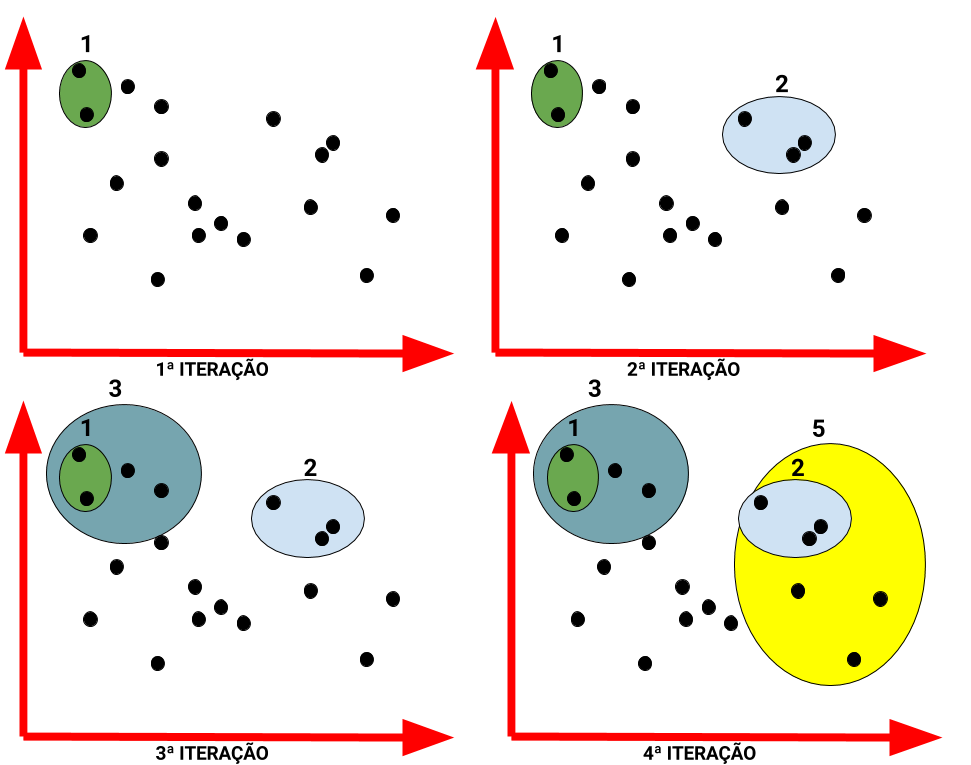
\includegraphics[width=12cm]{figuras/processo-aglomerativo}}
	}{
		\Fonte{Autoria própria.}		
	}	
\end{figure}
\begin{figure}[ht!]
	\centering
	\Caption{\label{fig:proc-div} Iterações algoritmos divisivos}	
	\UECEfig{}{
		\fbox{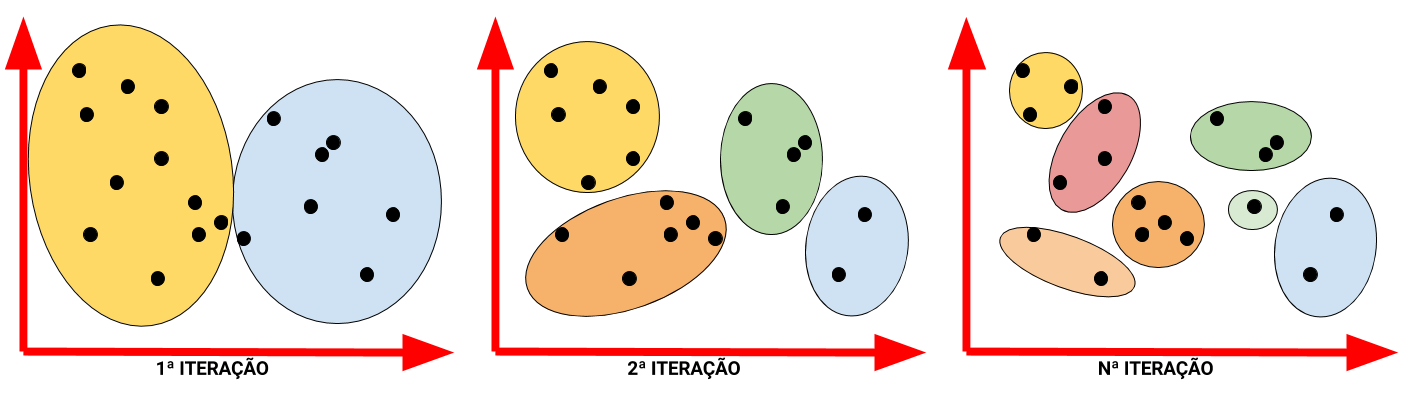
\includegraphics[width=14cm, height=4cm]{figuras/processo-divisivo}}
	}{
		\Fonte{Autoria própria.}		
	}	
\end{figure}

\begin{quadro}[h!]	
	\centering
	\Caption{\label{qua:k-means-str-wek} Vantagens e Desvantagens Algoritmo k-means}		
	\UECEqua{}{
		{\renewcommand{\arraystretch}{2}
		\begin{tabular}{|L{7cm}  L{7cm}|}
			\hline
			Vantagens & Desvantagens \\
			\hline
			\tabitem Utiliza principios simples para identificar \textit{clusters}, quais podem ser explicados
			em termos não estatísticos.
			
			
			\tabitem  É altamente flexísivel e tem a capacidade de se adaptar e com poucos ajustes sanar suas deficiências.
			
			
			\tabitem É muito eficiente e separa os dados em clusters uteis.		
			& 
			\tabitem É menos sofisticado que os algoritmos de clusterização mais recentes.


			\tabitem Por usar elementos aleatórios para treino, não há garantia de encontrar os melhores \textit{clusters}.
			
			
			\tabitem Requer um parâmetro assertivo sobre a quantidade de clusters existentes no conjunto de dados. 
			\\
			\hline
		\end{tabular}
		}
	}{
		\Fonte{Autoria própria.}
	}
\end{quadro}
